	\large \bf{\textsc{\section{Lab 3}}
	\begin{problem}
		Choose a diode type 1N4001 and build the following circuit.\\	
		R=100 \(\Omega\) (potentiometer) \\ 
		D is 1N4001 \\
		E=2v (max current I$_{max}$=350mA)
		\newline\newline
		1. Measure the diode and resistor voltage and current when changing the resistor R and fill the table
		\newline
		2. Plot the I-V characteristics  of the diode as well as the resistor. Are all measurements on one line? Are the components linear? Compare the diode i-v plot with the datasheet.
		\iffalse
			\begin{figure}[h!]
				\centering
				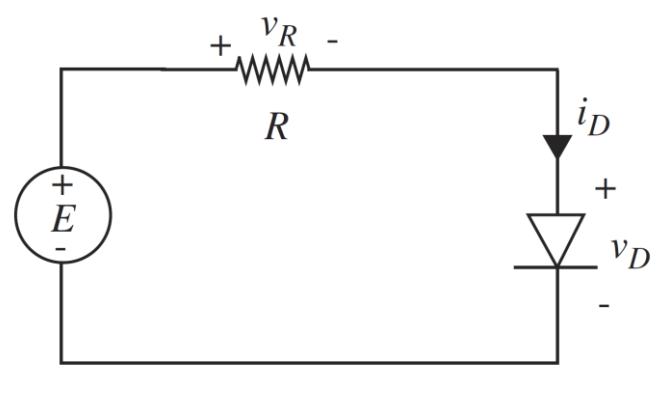
\includegraphics[width=0.5\textwidth]{images/circuit1.png}
			\end{figure}
		\fi
	\end{problem}
	
	\begin{solution}
		1.
		\begin{table}[h]
			\begin{tabular}{| l | l | l | l | l | l | l | l | l | l | l | l |}
				\hline
				Try          & 1 & 2 & 3 & 4 & 5 & 6 & 7 & 8 & 9 & 10 & 11 \\ \hline
				R (\(\Omega\))   & 64 & 60 & 55 & 42 & 23 & 13 & 8 & 5 & 4 & 2 & 1  \\ \hline
				V$_{D}$ (V)      & 0,7 & 0,712 & 0,72 & 0,723 & 0,742 & 0,783 & 0,789 & 0,833 & 0,88 & 0,824 & 0,855    \\ \hline
				V$_{R}$ (V)  & 1,33 & 1,32 & 1,31 & 1,3 & 1,28 & 1,17 & 1,12 & 1,105 & 0,99 & 0,79 & 0,67  \\ \hline
				i$_{D}$ (mA) & 20 & 30 & 50 & 80 & 120 & 160 & 200 & 240 & 280 & 320 & 350 \\ \hline
			\end{tabular}
		\end{table}
		\newline
		2.
		\begin{figure}[h!]
			\centering
			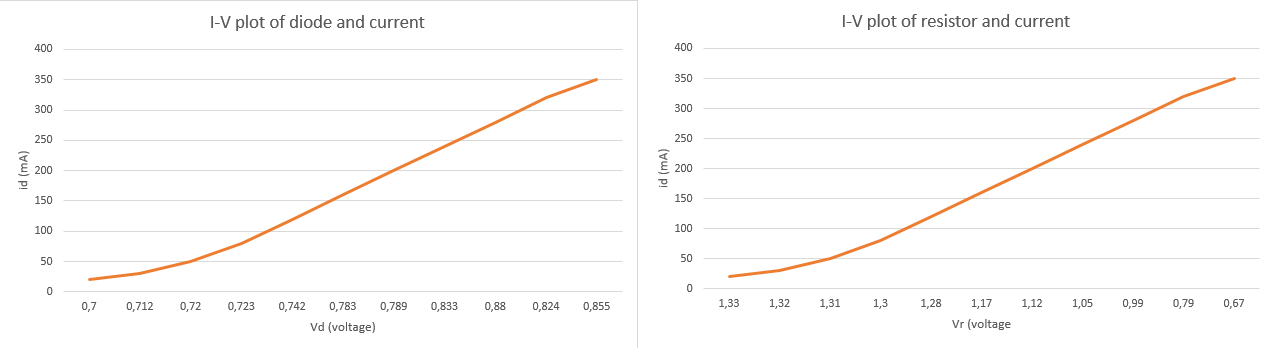
\includegraphics[width=1\textwidth]{images/ivlab3.png}
		\end{figure}
		All the measurements are on the line and it's comparable to the given I-V plot of the datasheet for the diode  
	\end{solution}
	\clearpage
	\begin{problem}
		In this exercise, we would like to build a full wave rectifier using a diode bridge.
		\newline
		1. Construct the following circuit using:\\
		R\(_{L}\)=10K\(\Omega\)\\
		D is 1N4001\\
		V\(_{i}\)=20sin(100\(\pi\)t)\\
		\newline
		2. Measure the input voltage and current using a multimeter.
		\newline
		3. Measure the output voltage on R\(_{L}\) using a multimeter and an oscilloscope.
		\newline
		4. Compare the measurements with your calculations
		\newline
		5. (Optional) Use a 470\(\mu\)F capacitor in parallel with R\(_{L}\) and measure the output voltage.
		\iffalse
			\begin{figure}[h!]
				\centering
				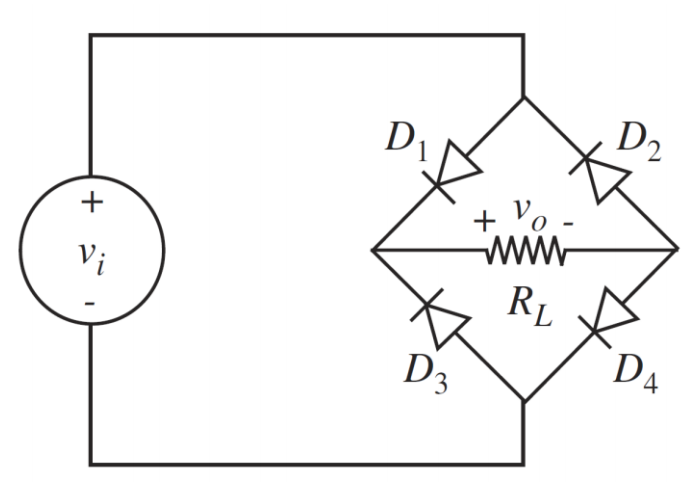
\includegraphics[width=0.5\textwidth]{images/circuit2.png}
			\end{figure}
		\fi
	\end{problem}
	
	\begin{solution}
		2. We measured it to be 14.3V and current to be 1.28mA
		\begin{figure}[h!]
			\centering
			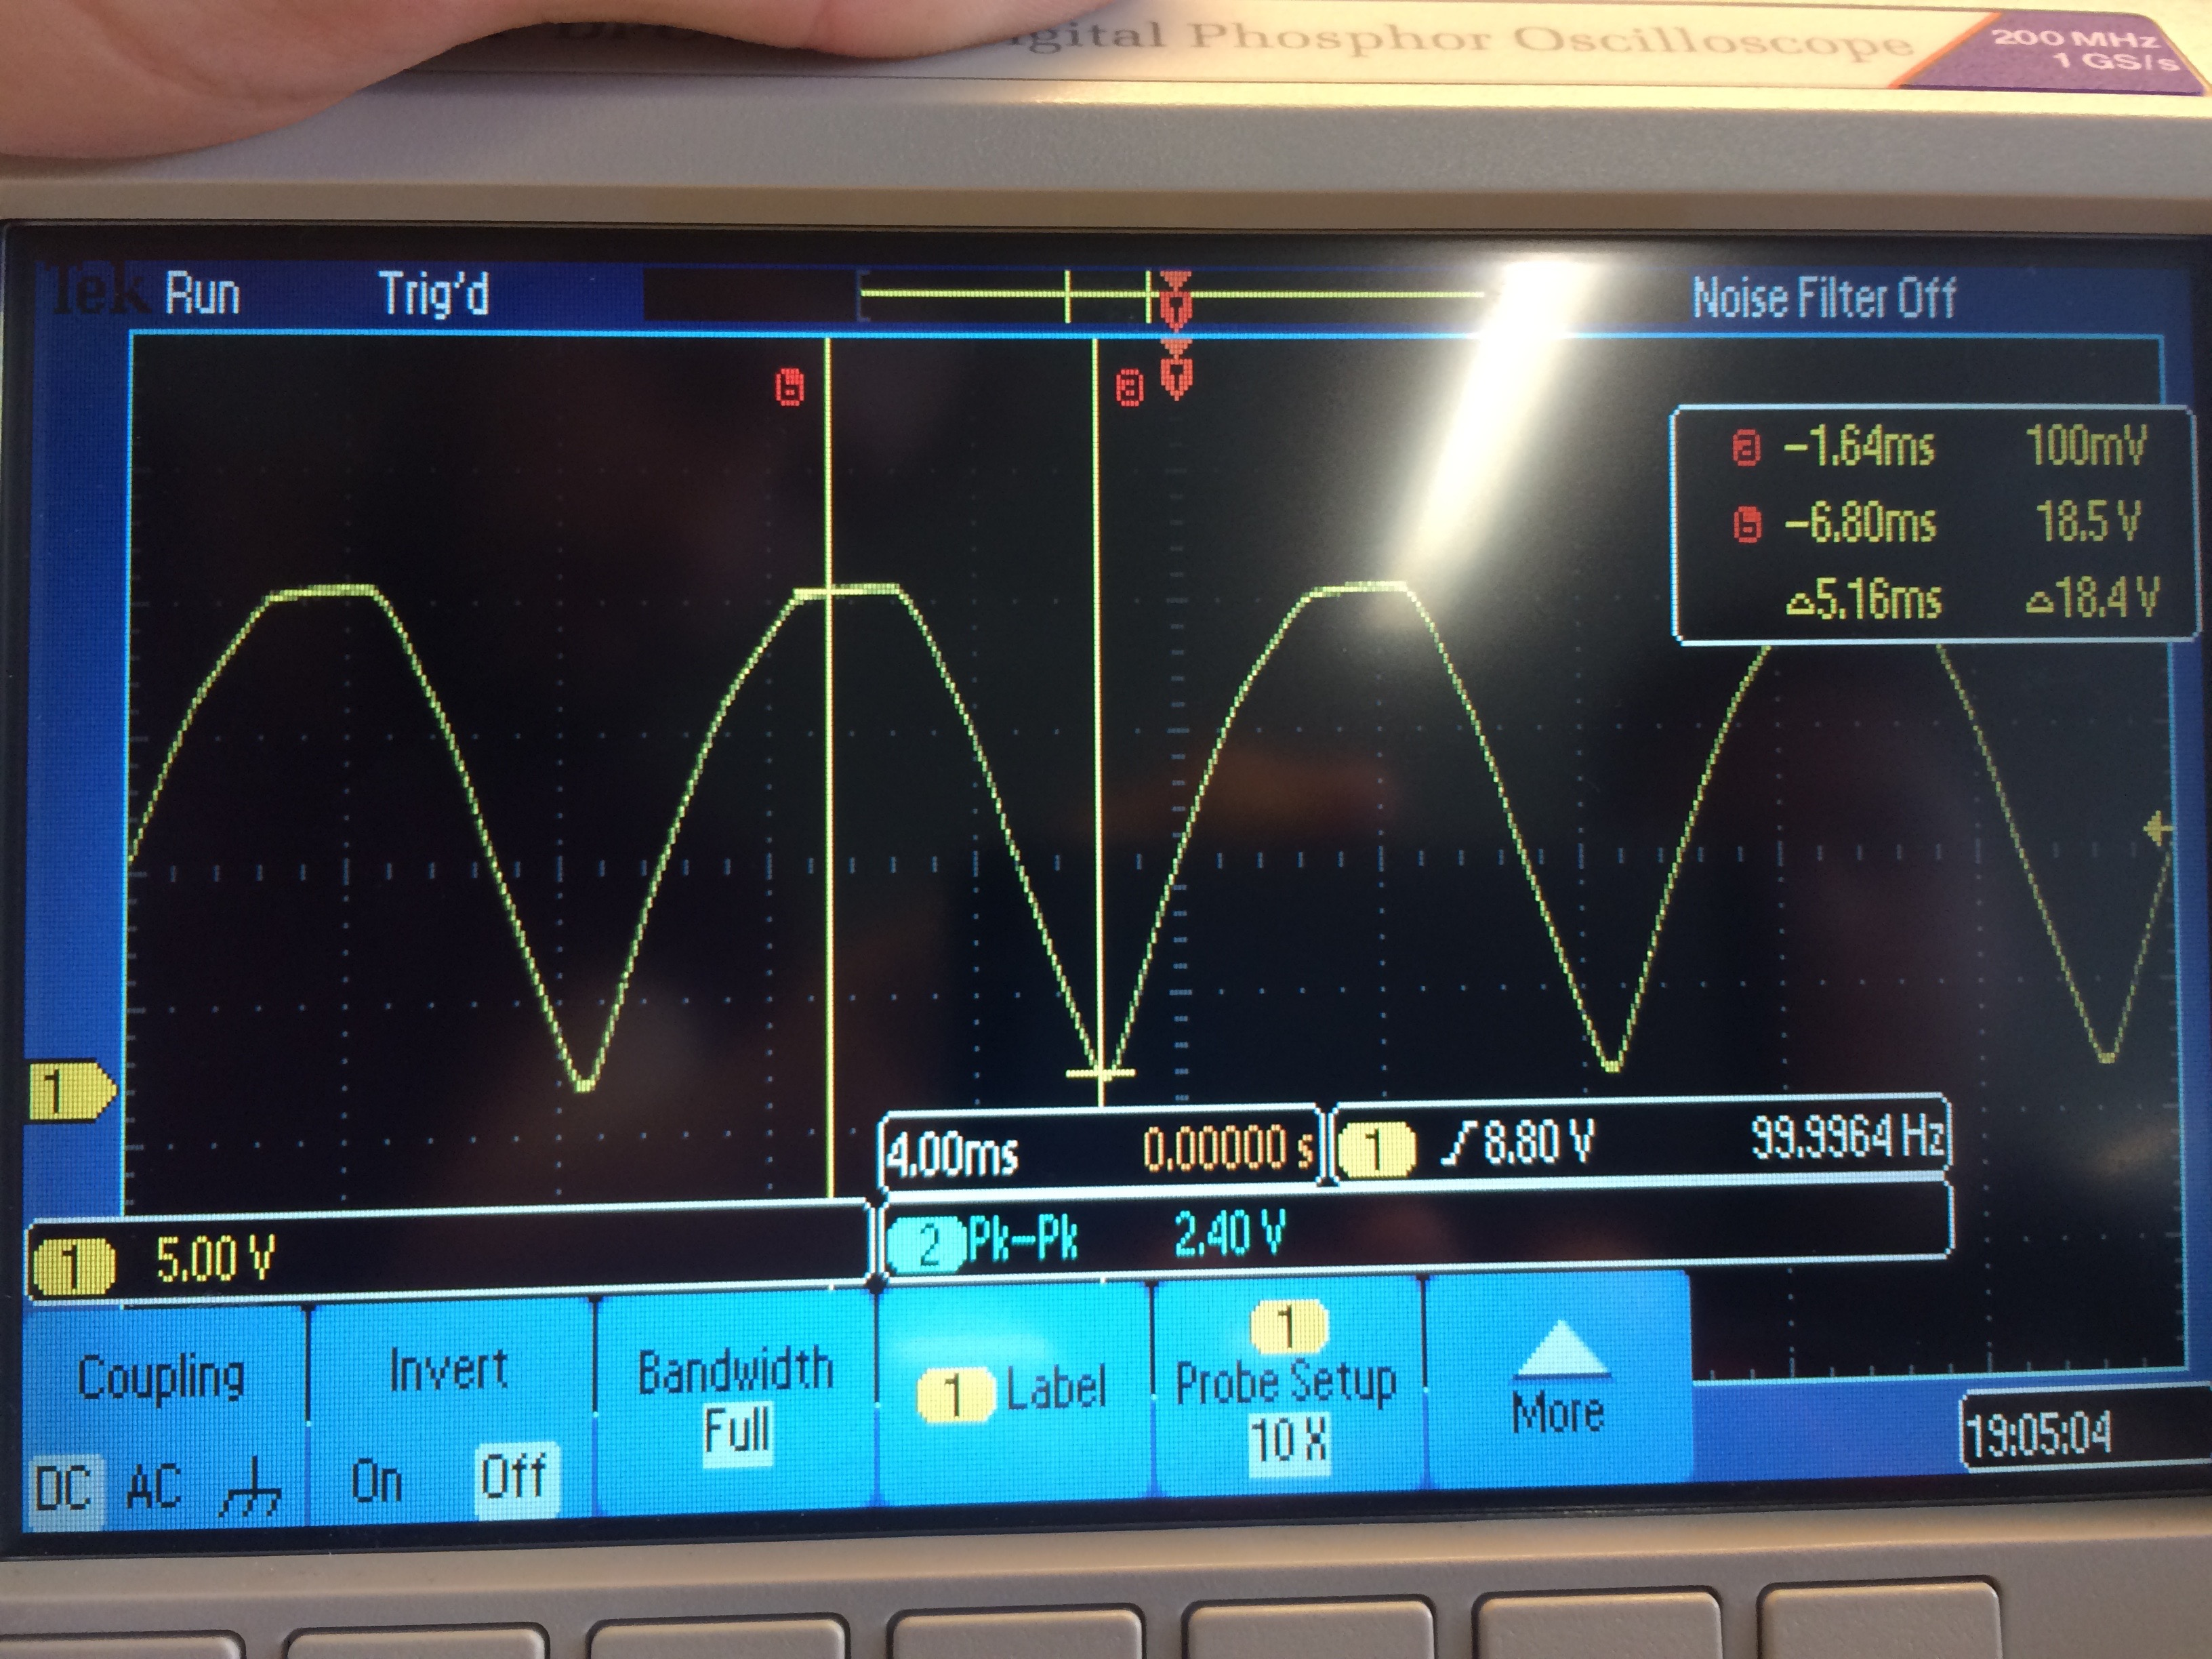
\includegraphics[width=0.45\textwidth]{images/plot323.jpg}
		\end{figure}
		\newline
		3. The oscilloscope measured 19.2V and the multimeter 12V
		\newline
		4. \[ V_{DC}=V_{AV}=2V/pi 
			  V_{DC}=2*19.2V/4.14=12.2V		\]
		The measurements are the same as the calculations. = 12V 		
		\newline
		5. We measured R\(_{L}\) to be 18.37 and a constant DC. Resistor is big = uses small current and the "tank" is full.
		\begin{figure}[h!]
			\centering
			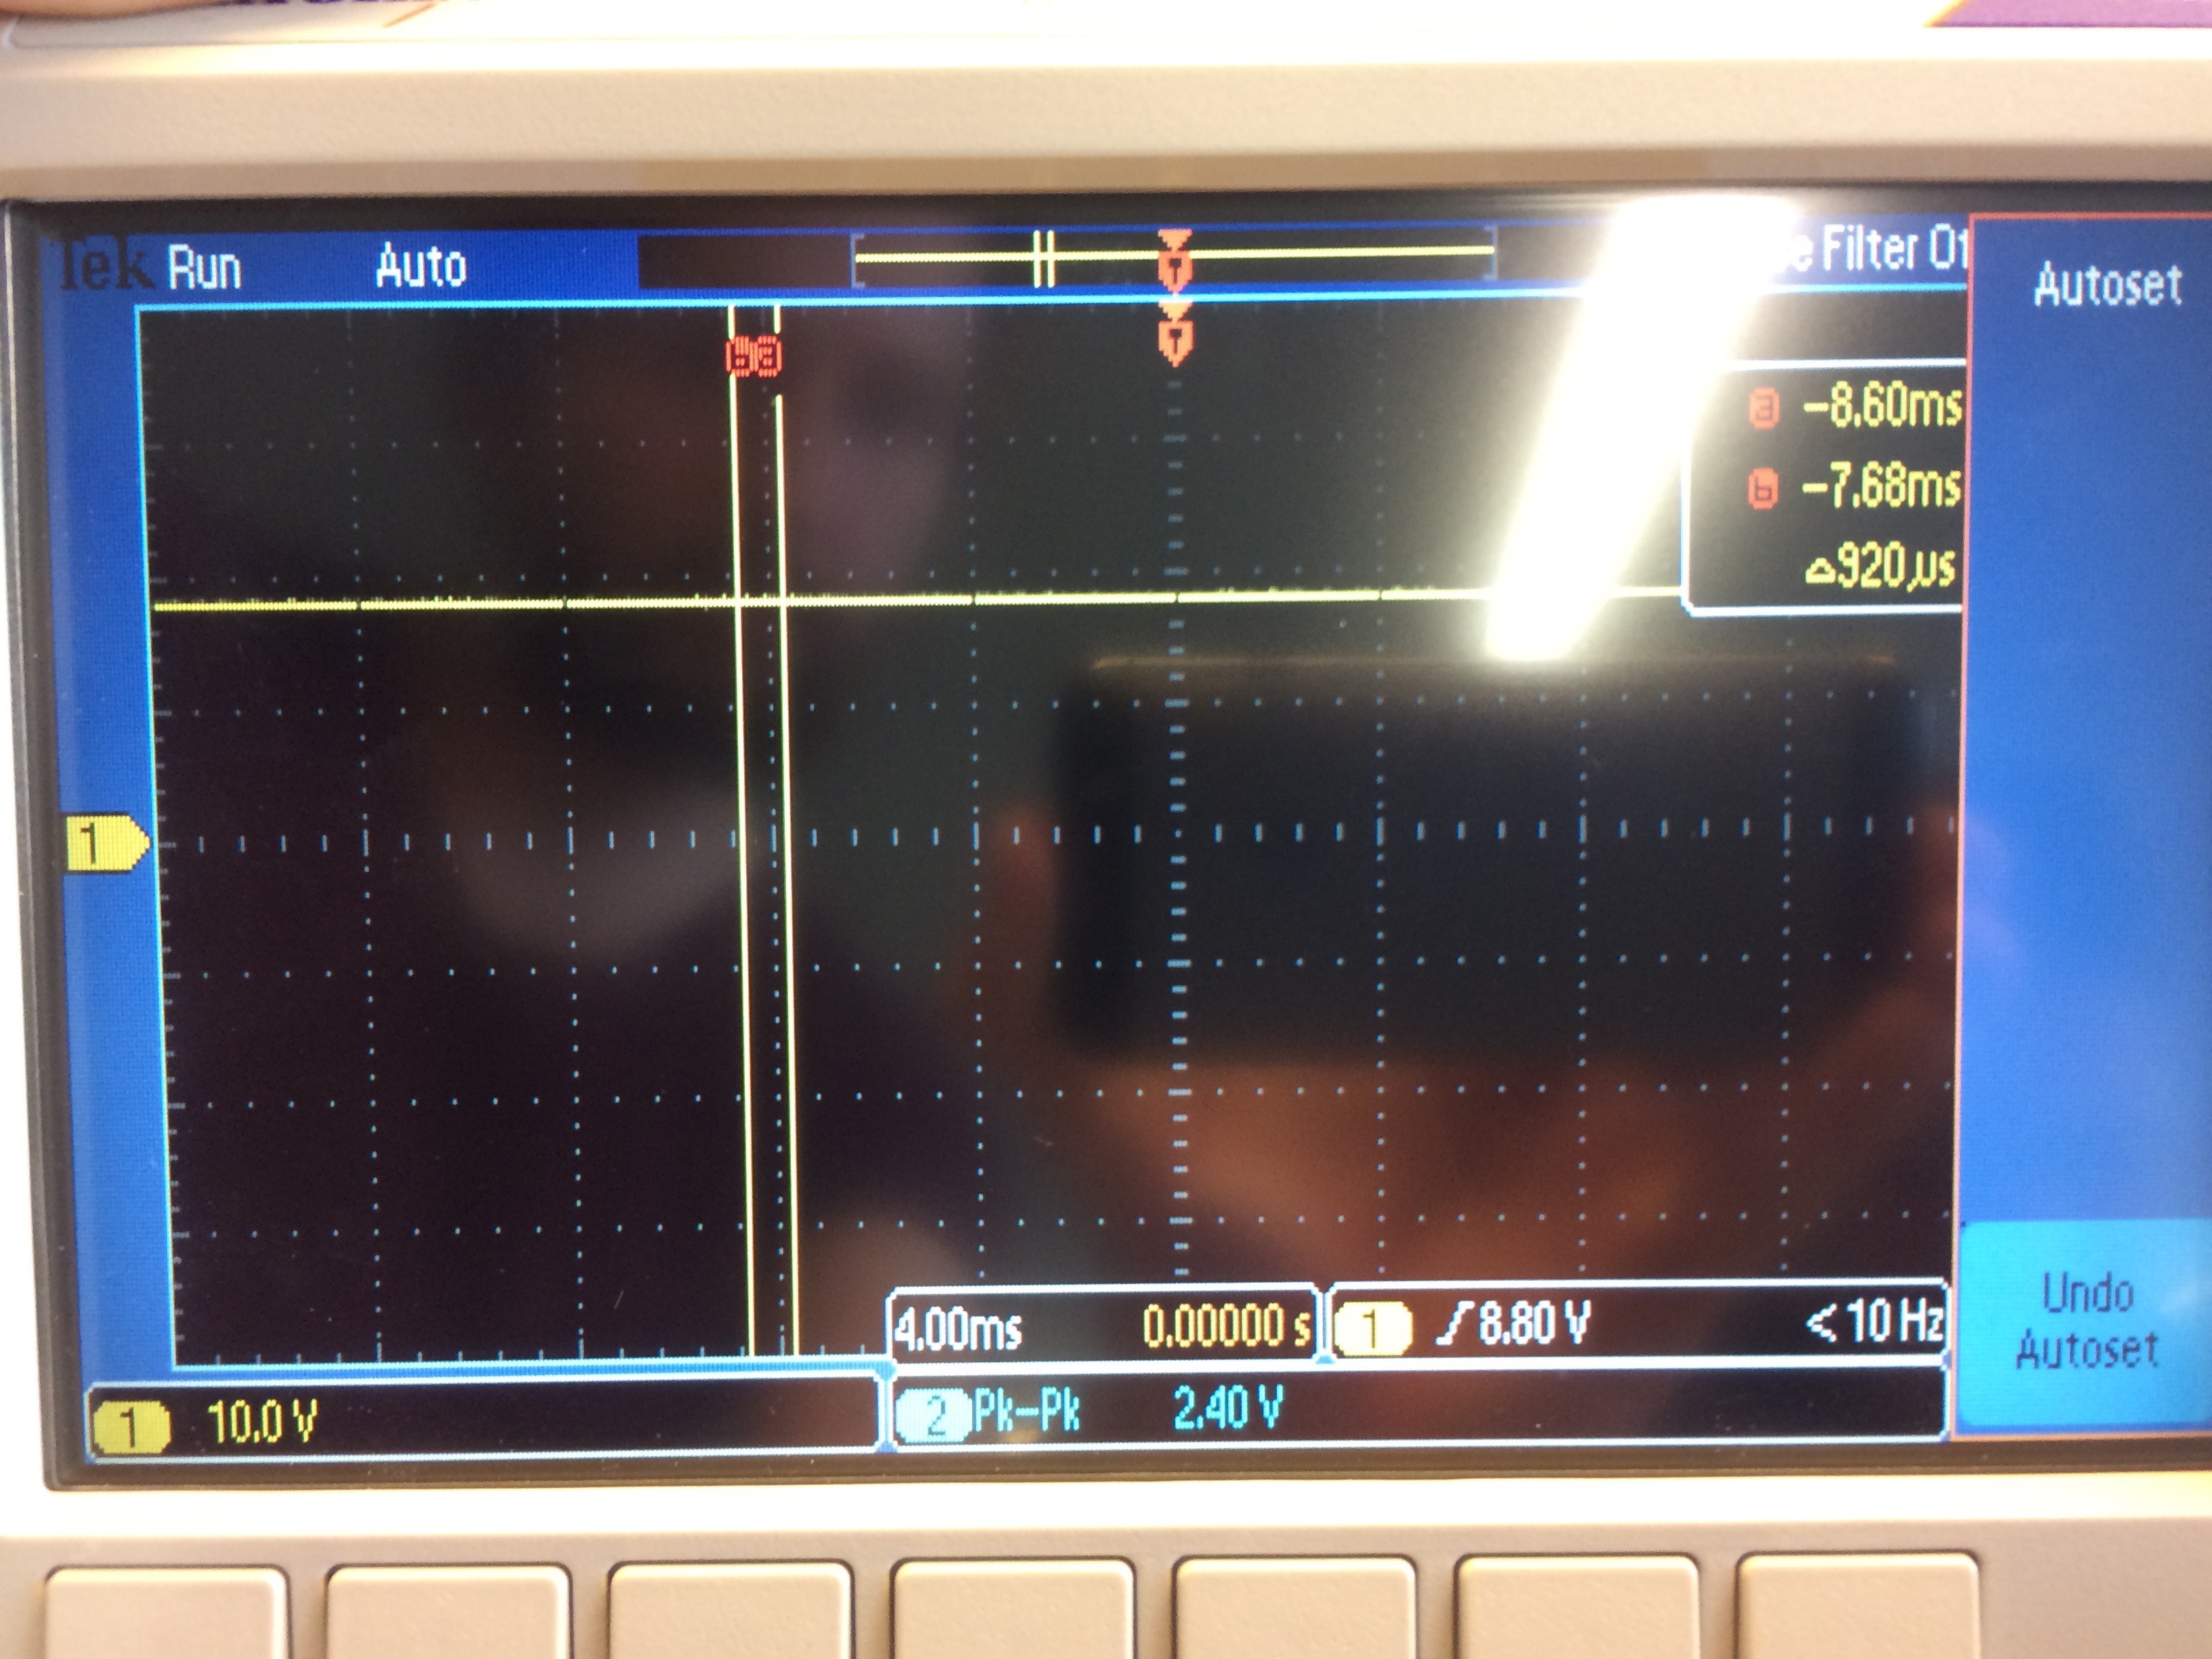
\includegraphics[width=0.45\textwidth]{images/plot325.jpg}
		\end{figure}
	\end{solution}
	\clearpage
	\begin{problem}
		Using an OpAmp TL082, construct an inverting amplifier of gain 2.
		\newline
		V\(_{i}\)=1.5v\\
		V\(_{CC}\)=12v\\
		Output current should not exceed 10mA
		\newline
		1. Measure the output voltage and compare with your expectations.
		\newline
		2. Use V\(_{i}\)=2sin(100\(\mu\)t) and measure the output voltage using an oscilloscope.
		\begin{figure}[h!]
			\centering
			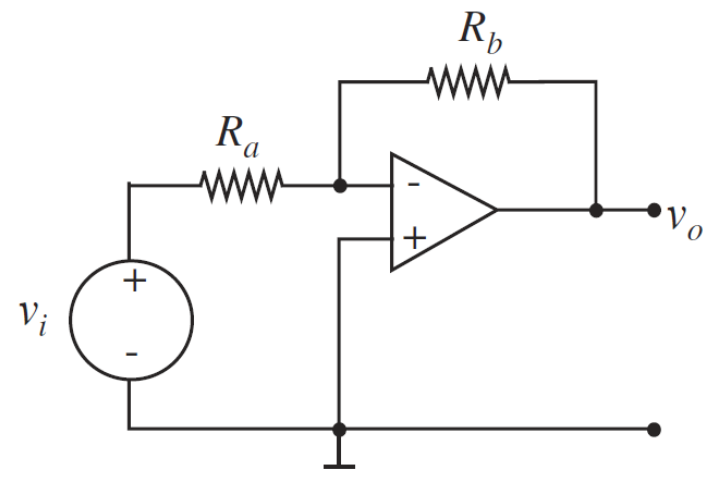
\includegraphics[width=0.5\textwidth]{images/circuit3.png}
		\end{figure}
	\end{problem}
	
	\begin{solution}
		1. -R\(_{f}\)/R\(_{in}\)*1.5=-2,97V, R\(_{f}\)=5.6K\(\Omega\) and R\(_{in}\)= 11.1K\(\Omega\). We measured -3.188V. The error comes from the resistors not giving a gain that is exactly 2, plus that the resistors are not exactly their given resistance. Adding up those errors should come close to difference in calculation and measurement.
		\newline
		2.  V\(_{o}\)= 1.7V rms. It should have been 1.4V rms. The error in measurement could have come from our setup and our inexperience with the use of oscilloscope.
	\end{solution}